\title{Simulation of Shock Tube Flows with an Adaptive Conservative Scheme}
\author{} \institute{}
\tocauthor{\underline{D.~Isola}, A.~Guardone}
\maketitle

\begin{center}
{\large \underline{Dario Isola}, Alberto Guardone}\\
Dipartimento di Ing. Aerospaziale, Politecnico di Milano\\
{\tt isola@aero.polimi.it, guardone@aero.polimi.it}
\end{center}

\section*{Abstract}
The numerical simulation of two-dimensional shock tube flows can be particularly challenging since, even in simple geometries, very complex unsteady flows can develop~\cite{Woodward-Colella-1984}. A quite common feature of such flows is the presence of moving shocks separating regions where the flow is substantially uniform. To reduce the computational burden and improve the overall accuracy of the solution, mesh adaptation techniques can be adopted to increase the grid spacing only where it is required~\cite{Naderi-Darbandi-Rahni-2010}.  In the present work a Finite-Volume solver for the Arbitrary Lagrangian-Eulerian (ALE) formulation of the Euler equations over two-dimensional adaptive grids~\cite{Forestieri-Isola-Marulli-Guardone-Quaranta-2010} is adopted to perform unsteady flow computations. The interpretation of the grid modifications as a continuous deformation of the finite volumes, resulting in a modification of the interface velocities, allows to compute the solution onto the new grid simply integrating the governing equations, without any explicit interpolation step~\cite{Isola-Guardone-Quaranta-2010}.

\begin{figure}
\centering
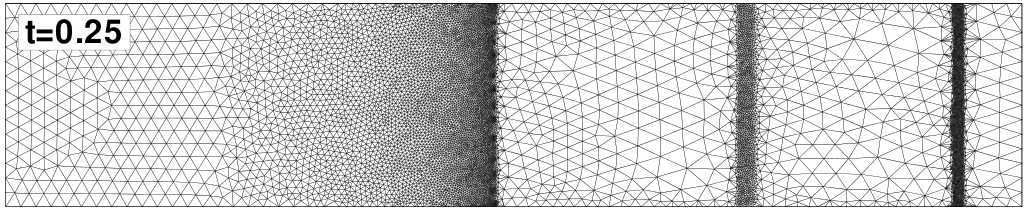
\includegraphics[height=.16\textwidth]{./isola/grid.png}
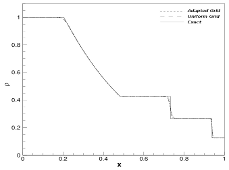
\includegraphics[height=.16\textwidth]{./isola/solution.png}
\caption{Adapted grid and density along the shock tube.}
\end{figure}

\bibliographystyle{plain}
\begin{thebibliography}{10}
\bibitem{Woodward-Colella-1984}
{\sc P.~Colella and P.~R.~Woodward}. {The numerical simulation of two-dimensional fluid flow with strong shocks}. J. Comput. Phys. (Elsevier) 54: 115--173, (1984).
	
\bibitem{Naderi-Darbandi-Rahni-2010}
{\sc A.~Naderi, M.~Darbandi and M.~Taeibi-Rahni}. {Developing a unified FVE-ALE approach to solve unsteady fluid flow with moving boundaries}. {International Journal for Numerical Methods in Fluids, 63(1):40--68, (2010).}
	
\bibitem{Forestieri-Isola-Marulli-Guardone-Quaranta-2010}
{\sc G.~Forestieri, D.~Isola, F.~Marulli, G.~Quaranta and A.~Guardone}. {Numerical simulation of compressible vortical flows using a conservative unstructured-grid adaptive scheme}. 2$^{nd}$ European Seminar on Coupled Problems, Pilsen, Czech Republic, (28$^{th}$ June -2$^{nd}$ July, 2010).
	
\bibitem{Isola-Guardone-Quaranta-2010}
{\sc D. Isola, A. Guardone, and G. Quaranta}. {An {ALE} scheme without interpolation for moving domain with adaptive grids}. AIAA 40\ensuremath{^{\textrm{th}}} Fluid Dynamics Conference and Exhibit, Chicago, IL, USA, (28 June--1 July 2010).
\end{thebibliography}
